%
% Introduction
%
\section{Introduction}
Web-crawling is used for collecting data in various fields. Some web-crawlers collect data even though the site is preventing crawlers by robot.txt. This can have a serious impact on the availability of the target service. These web-crawlers modify the header value, distribute IP to masquerade as if they are legitimated users to prevent themselves from detection.
It is also prohibited to duplicate an entire dataset, even if the service permits viewing of individual data. However, malicious distributed web-crawlers browse and replicate the entire data of the service.
In this paper, we introduce the anti-crawling methods and its countermeasures, and show that the conventional anti-crawling method cannot defend the distributed crawler. We also introduce a new anti-crawling technique that gradually adds an IP set using a distributed crawler to the black-list.

%
% Back Ground
% with 2 subsections
%
\section{Related Works}
\begin{enumerate}

\item HTTP Header Check
\newline A basic crawler will send requests without modifying its header information. And web servers can distinguishes a legitimate user from a crawler by checking the request header, especially User-Agent value has been set properly. This header checking method is a basic anti-crawling method.
But if a crawler attempts to masquerade itself as a legitimate user, it will replay the header information from the web browser or form the http header information similar to a browser. This makes it difficult for a web server to determine whether a client is a crawler or a legitimate user by simply checking the request header.
\newline

\item Access Pattern based Anti-Crawling
\newline
Access pattern based anti-crawling is a method of classifying legitimate users and crawlers based on the pattern requested by the client. If a client requests only a specific resource continuously without a call to a resource that should normally be requested, the corresponding could be regarded as a crawler. 
An attacker performing an aggressive crawling predefines the core data that the web service wants to collect, and implements a crawler that requests specific data without requesting unnecessary resources. In this case, the web server can recognize that the client is not a legitimate user.
In the case of a web service using advanced approach to access pattern recognition, the service is viewed as a set of consecutive requests from the viewpoint of the user UX, and requests and responses belonging to the same set are chained by including a specific hash value in the cookie.
Although this approach can recognize a crawler based on access pattern, some crawlers even masquerade their access pattern by analyzing network logs.[Inwoo Ro] 
\newline 
\item Access Frequency based Anti-Crawling
\newline 
Access frequency based anti-crawling is a method that determines a client is whether a crawler or a legitimate user by access frequency rate. A web server can set a threshold limit of access count in an unit time. If a client with a specific IP requests exceeds this limit in pre-defined time, the web server determines that this IP as a crowler node.

This method has two well known problems. 
First, it has vulnerability against distributed crawler. If an attackers use distributed crawler such as Crawlera, access rate for a crawler node IP will be reduced enough to bypass threshold limit.
Second, it could raise false positive error if many users share a public IP.
\newline


\end{enumerate}


%
% BLOCKING DISTRIBUTED CRAWLER
% with 2 subsections
%
\section{BLOCKING DISTRIBUTED CRAWLER}
In this section, we propose a new technique to detect and block distributed crawlers that could not be defended by existing anti-crawling techniques.

\subsection{Number of Distributed Nodes}
In order for the Distributed crawler to replicate the historical data of a website, the following conditions must be met. Cn ≥ Um / (Td * 30) for the number of items (Um) updated in the target site on a month, the maximum number of connections (Td) per day restricted by the site, and the number of IPs (Cn) Must be satisfied.
For example, if a service that updates 60,000 data per month limits the maximum number of connections per day to 50, an attacker must perform crawling using at least 40 distributed IPs. Conversely, on the service provider side, the larger the Um, the smaller the Td is, the more advantageous it is. However, Um is difficult to secure arbitrarily, and if Td is reduced, the ratio of false positives to normal users increases.


\subsection{Node Reducing with statistical approach}
Instead of increasing the Um from the service provider side, or reducing the Td is a method of identifying a portion of the crawler to Cn and Cn by reducing the block.
Assuming that the number of IPs used by the attacker is Cm, the attacker must satisfy Cn - Cm ≥ Um / (Td * 30). On the service provider side, Cm satisfying Cm ≥ Cn - Um / (Td * 30) can be obtained.
Service providers can create a block-list without reducing Td in a batch by using statistical techniques. The frequency of access by users is not the same for each item, and when the items with the highest frequency of access are arranged on the left side, they are distributed in a graph form which exponentially decreases according to a power law as follows.

\begin{figure}[H]
    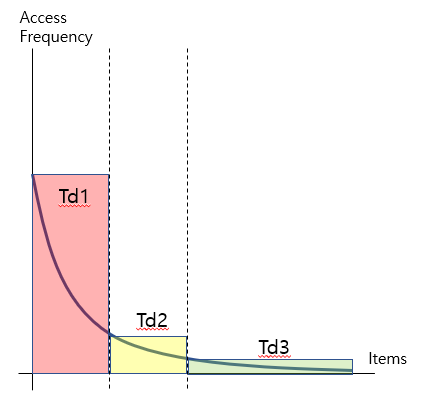
\includegraphics[width=1.0\columnwidth]{figs/figure_01.png}
    \caption{Access Frequency per number of connections}
    \label{fig:my_label}
\end{figure}

In order for an attacker to replicate historical data from the service, he must also access the items in the long-tail (Td3) interval. However, the attacker does not know exactly which item the item he is accessing belongs to. Using this information asymmetry, service providers can easily identify IPs that are accessed more frequently than long-tailed segments. If we start to increase the Cm value through the long-tail interval, the attacker will crawl with a smaller number of IPs, and Cm will increase in the Td2 interval.
The Td value for each interval is calculated by adding the standard deviation (s) of the corresponding interval access frequency to the access frequency value (Amax) of the item having the highest access frequency per IP among the corresponding interval items as follows. 

  \begin{displaymath}
    Td = Amax + s * 2
  \end{displaymath}

If a particular IP accesses an item in the long-tail region with more than the Td value determined by the above formula, it can be included in the block-list.

\subsection{Dummy Items}
The service provider may include a dummy item to detect the crawler in addition to the actual service target item. The item is normally inaccessible to the general user through the UI. For example, it exists as an HTML tag but it is not displayed on the screen due to the attribute setting or the case where the ordinary user is not interested because it exists on the index but is not in the real world.
Such a dummy item may approach a crawler that performs sequential access but it can maintain a relatively low threshold value because the accessibility of the general user is low and it generates a lower interval than the long-tail interval derived from the traffic can do.



%
% EXPERIMENT
%
\section{EXPERIMENT}
In order to verify the above, experiments were performed to classify the crawler IP for the actual web traffic data. It is based on the web traffic of 1 month released by NASA. Details and experimental method of data are as follows.


\subsection{Web Traffic Data}


\begin{enumerate}
\item Source
\newline NASA released a total of 1,891,715 access logs for the month of July 1995. In this paper, the log is parsed into csv format and composed of 4 columns including IP, date, access target and access result.
The total number of connected IPs is 81,978 and the number of items is 21,649. The most accessed items received 111,116 requests as '/images/NASA-logosmall.gif'.
\newline
\item Traffic Distribution
\newline 
The total number of accesses is calculated for each access target, and the sorting is performed in order of the largest number of connections. The results are confirmed to be distributed in a form in which a power law is applied as described in Section 5. 
In addition, as shown in Figures 2, 3 and 4, power distribution is also observed internally in Td1, Td2, and Long-tail sections. Figurue 2 is a graph of connection frequency of 38 items corresponding to the upper 0.5\% of Td1, Figure 3 shows the top 100 ~ 2000 figures corresponding to Td2, Figure 4 shows the frequency of 100 ~ 2000 . In the next section of the simulator, node reduction will be performed using a set of items belonging to the long-tail as described above.
\end{enumerate}

\begin{figure}[H]
    \centering
    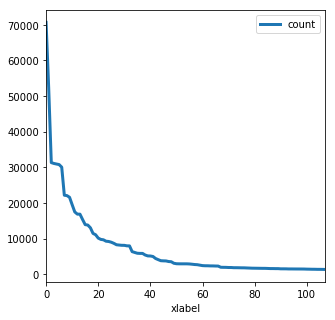
\includegraphics[width=0.7\columnwidth]{figs/figure_02_td1.png}
    \caption{Access Count in Td1}
    \label{fig:my_label}
\end{figure}

\begin{figure}[H]
    \centering
    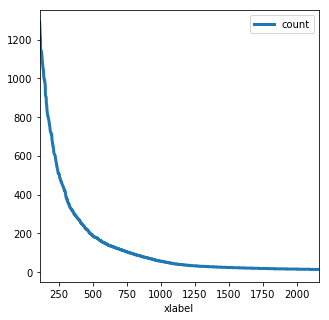
\includegraphics[width=0.7\columnwidth]{figs/figure_03_td2.png}
    \caption{Access Count in Td2}
    \label{fig:my_label}
\end{figure}

\begin{figure}[H]
    \centering
    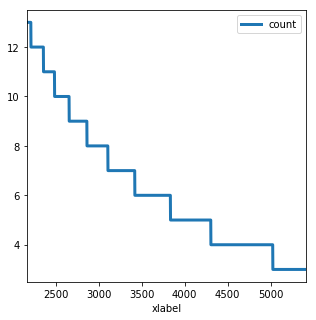
\includegraphics[width=0.7\columnwidth]{figs/figure_04_td3.png}
    \caption{Access Count in Long-tail}
    \label{fig:my_label}
\end{figure}

\subsection{Simulation}
In this paper, we implemented two kinds of simulation. One is to check whether it is possible to detect and disable the crawler IP group by performing node reduction through items belonging to the long-tail, and the other is to check false positive when the actual traffic is input to the same detection logic .


\begin{enumerate}
\item Data Pre-Processing
\newline In order to prevent duplication of data used in modeling and experimental data in the time series data, Long-tail was constructed by using data from 1 to 24 days in 30 matching data. Traffic verification was performed from the 25th to the last day Data. \& Lt; / RTI \& gt;
When accessing html files, gif extension files are removed from the long-tail group in order to prevent cumulative access values from increasing in duplicate while accessing gif extension files together.
Finally, the request log which was not accessed successfully was excluded from the experiment.
\newline
\item Simulators
\newline 
The simulator is implemented using python. The parameters are the size of the distributed IP set used by the crawler, the long-tail list, the entire item list, and threshold values used for detection.
The implementation method allows the Crawler IP Set to access each item by traversing the entire item list, and accesses the IP in the crawler distributed IP set at each access.
When the crawler accesses a long-tail entry, it adds the IP to the warning dictionary and increments the access count by one. However, if the same IP accesses the same item, it does not increase the access count because it is not related to the purpose of crawling. When the access count exceeds the threshold value, Node Reducing is implemented by adding the corresponding IP to the banned list. Figure 5 below shows an example of running a crawler using 100 distributed IPs for 7,649 items. The number of long-tail items is 5,355 and the threshold is set to 20. 

\begin{figure}[H]
    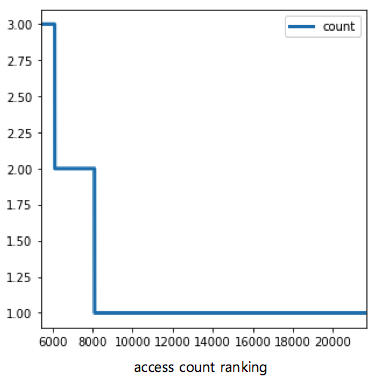
\includegraphics[width=0.65\columnwidth]{figs/figure_05_td4.png}
    \caption{Number of IPs using crawling}
    \label{fig:my_label}
\end{figure}

The IPs included in the crawler IP set gradually accumulate the access count, and the node reduction starts from the point when the access count of the entire crawler node group increases beyond {number of nodes} * {threshold}.
Another function of the simulator is to input the request request to the crawler simulator based on the actual web traffic log. This is implemented to confirm the case where the simulator judges the actual web traffic as a crawler.
\newline
\item Node Reducing Result
\newline 
Experiments were performed with threshold set to 30, and the crawler set consisting of up to 222 nodes was completely detectable. If the number of nodes exceeded 300, it was not detected at all. False positives were 1.33 cases per day, which was 0.0312\% of the daily average IP number of 3,631. The following figure is a graph of the process of reducing 222 crawler sets on the simulator.

\begin{figure}[H]
    \centering
    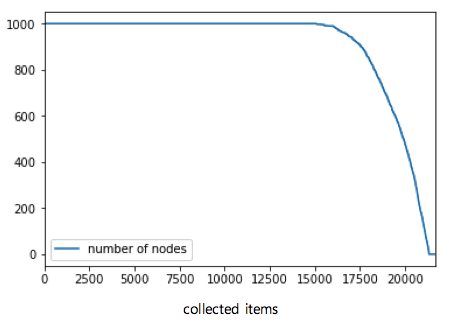
\includegraphics[width=0.7\columnwidth]{figs/figure_06_nr.png}
    \caption{Number of IPs reduced by detection}
    \label{fig:my_label}
\end{figure}

This is based on NASA traffic data in 1995, and can be applied to more or less crawler sets depending on the number of items the site has or the length of the long tail.
False positives occurred in 8 out of 6 matching data and 6 IPs were recognized as crawler nodes except duplicate detection. The number of requests generated per month for each IP is as follows.


\begin{table}
  \caption{IP and domains generated requests}
  \label{tab:freq}
  \begin{tabular}{ccl}
    \toprule
    IP or domain&Port\\
    \midrule
    156.80.168.122 & 117\\
    163.205.180.17 & 564\\
    dwkm206.usa1.com & 167\\
    jalisco.engr.ucdavis.edu & 424\\
    jbiagioni.npt.nuwc.navy.mil & 2124\\
    sputnix.cas.und.nodak.edu & 101\\
  \bottomrule
\end{tabular}
\end{table}


156.80.168.122 and sputnix.cas.und.nodak.edu, which generated relatively few requests, were detected as crawler nodes because the requests of these IPs were concentrated on a certain date, 29.7\% of them were in the long-tail area Of the respondents.

\end{enumerate}



%
% CONCLUSION
%
\section{CONCLUSION}
In this paper, we introduce a node reducing method that identifies the IP set of distributed crawlers and gradually reduces IP by using the property that web traffic follows the power law.
The node reducing scheme has shown a very low level of false positives against distributed crawlers using multiple IPs, effectively identifying crawler sets.



%
% FUTURE WORKS
%
\section{FUTURE WORKS}
Web traffic generally tends to generate traffic bursts at certain times. [1] Although the experiment of this paper is based on actual traffic log, since the time point of the data used in the experiment is one month, it does not include cases where a new item is added or an issue occurs and a traffic burst occurs.
In order to apply the results of this paper more securely to actual services, it is necessary to study whether the item movement level and threshold value of long-tail area can be maintained based on actual traffic data for traffic burst occurrence cases.



%
% REFERENCES
%
\section{REFERENCES}
[1]	M.V Simkin and V.P. Roychowdhury, “A theory of web traffic” https://arxiv.org/pdf/0711.1235.pdf
\newline[2] Density Estimation for Statistics and Data Analysis
\newline[3] Explaining World Wide Web Traffic Self-Similarity
\newline[4] Research on Detection Algorithm of WEB Crawler
\newline[5] Design and Implementation of Scalable, Fully Distributed Web Crawler for a Web Search Engine
\newline[6] Design and Implementation of a Distributed Crawler and Filtering Processor
\newline[7] URL Assignment Algorithm of Crawler in Distributed System Based on Hash
\newline[8] Design and Implementation of a High-Performance Distributed Web Crawler
\newline[9] Feature evaluation for web crawler detection with data mining techniques
\newline[10] Crawler Detection: A Bayesian Approach
\newline[11] Real-time Web Crawler Detection
[12] An investigation of web crawler behavior: characterization and metrics


% Bibliography
\bibliographystyle{ACM-Reference-Format}
\bibliography{sambib}

